\documentclass[a4paper, 11pt, titlepage]{jsarticle}
\usepackage[dvipdfmx]{graphicx}
\usepackage{listings}
\usepackage{amsmath}
\usepackage{comment}

\title{知能情報基礎演習II \\ 要件定義と基本設計家書の作成 \\ グループ番号7 Develoop}
\author{245429H 末吉 良多 \\ 245745J 知念 拓弥 \\ 245704B 武嶋 優海}
\date{\today}

\begin{document}
\maketitle

\clearpage

\section{開発するアプリ名、内容、開発の背景等}%----------------------------------------------------------------------------------------------
\subsection{開発するアプリ名}
Shelfie
\subsection{内容}
自分が読んだ本、買った本の写真を撮り、デジタル本棚を作る
\subsection{開発背景}
多くの人が、読書を通じて得た感動や知識の証として、読んだ本をコレクションしたいという思いを持っています。\\
しかし、特に一人暮らしの学生など、限られたスペースや予算で生活する人々にとって、物理的な本棚を充実させていくことは簡単なことではありません。

「本は好きだけれど、置き場所がないから買えない」

「思い出深い本でも、泣く泣く手放さなければならない」\\
こうした悩みを解決し、誰もが気軽に自分だけの本棚を持てるようにしたいと思い開発を始めました。

\subsection{利用者のペルソナ}
\textbf{田中美咲}
\begin{itemize}
    \item \textbf{基本情報:} 20歳、大学3年生(文学部)。東京都内のワンルームで一人暮らし。
    \item \textbf{性格:} 感受性が豊かで、一人の時間を大切にする。自分の好きな作家や世界観には強いこだわりを持つ。
    \item \textbf{ライフスタイル:} 古本屋巡りが趣味。情報収集は主にSNSの読書アカウントから。
    \item \textbf{読書スタイル:} 装丁の美しい本を「モノ」として所有したい「紙の本派」。純文学や海外小説を好む。
    \item \textbf{ITリテラシー:} アプリの利用に抵抗はなく、直感的でおしゃれなデザインを好む。
    \item \textbf{課題:} 部屋が狭く本の置き場所に困っており、愛着のある本も手放さざるを得ない。
    \item \textbf{インサイト:} 手放した本も含め、読んだ証を「自分だけの本棚」として視覚的にコレクションしたい。
\end{itemize}

\clearpage

\subsection{ロゴ}
\begin{figure}[htbp]
\centering

\includegraphics[width=60mm] {shelfie_logo.png}
\label{fig:func}
\end{figure}

\begin{figure}[htbp]
\centering

\includegraphics[width=60mm] {shelfie_logo2.png}
\label{fig:func}
\end{figure}

\clearpage

\section{要件定義書}%----------------------------------------------------------------------------------------------
\begin{figure}[htbp]
\centering
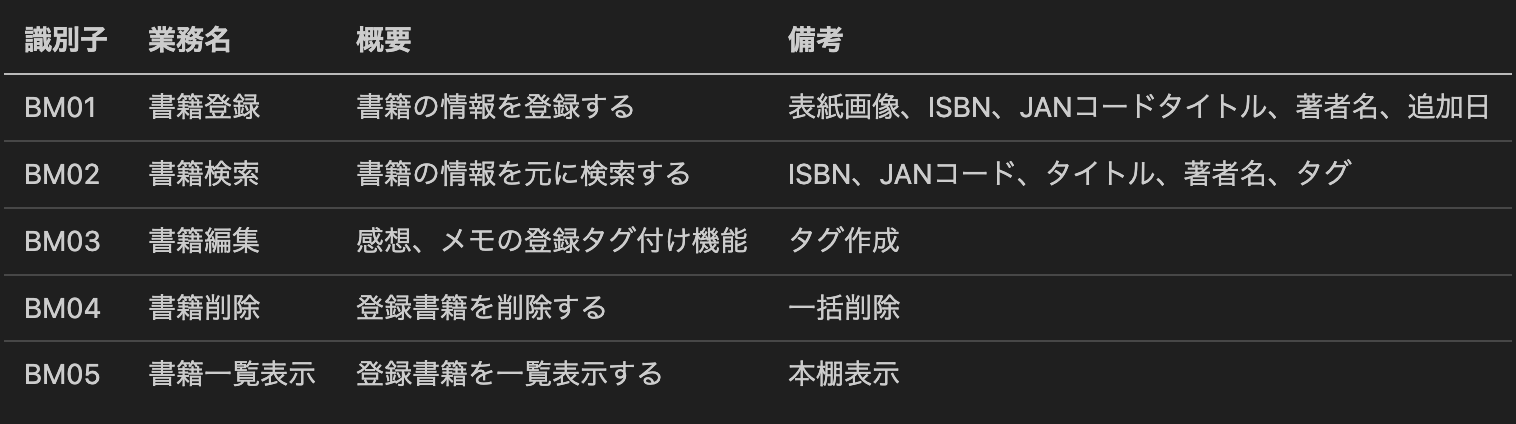
\includegraphics[width=120mm]{work.png}
\label{fig:func}
\end{figure}



\section{基本設計書}%----------------------------------------------------------------------------------------------
\subsection{基本機能}
\begin{figure}[htbp]
\centering
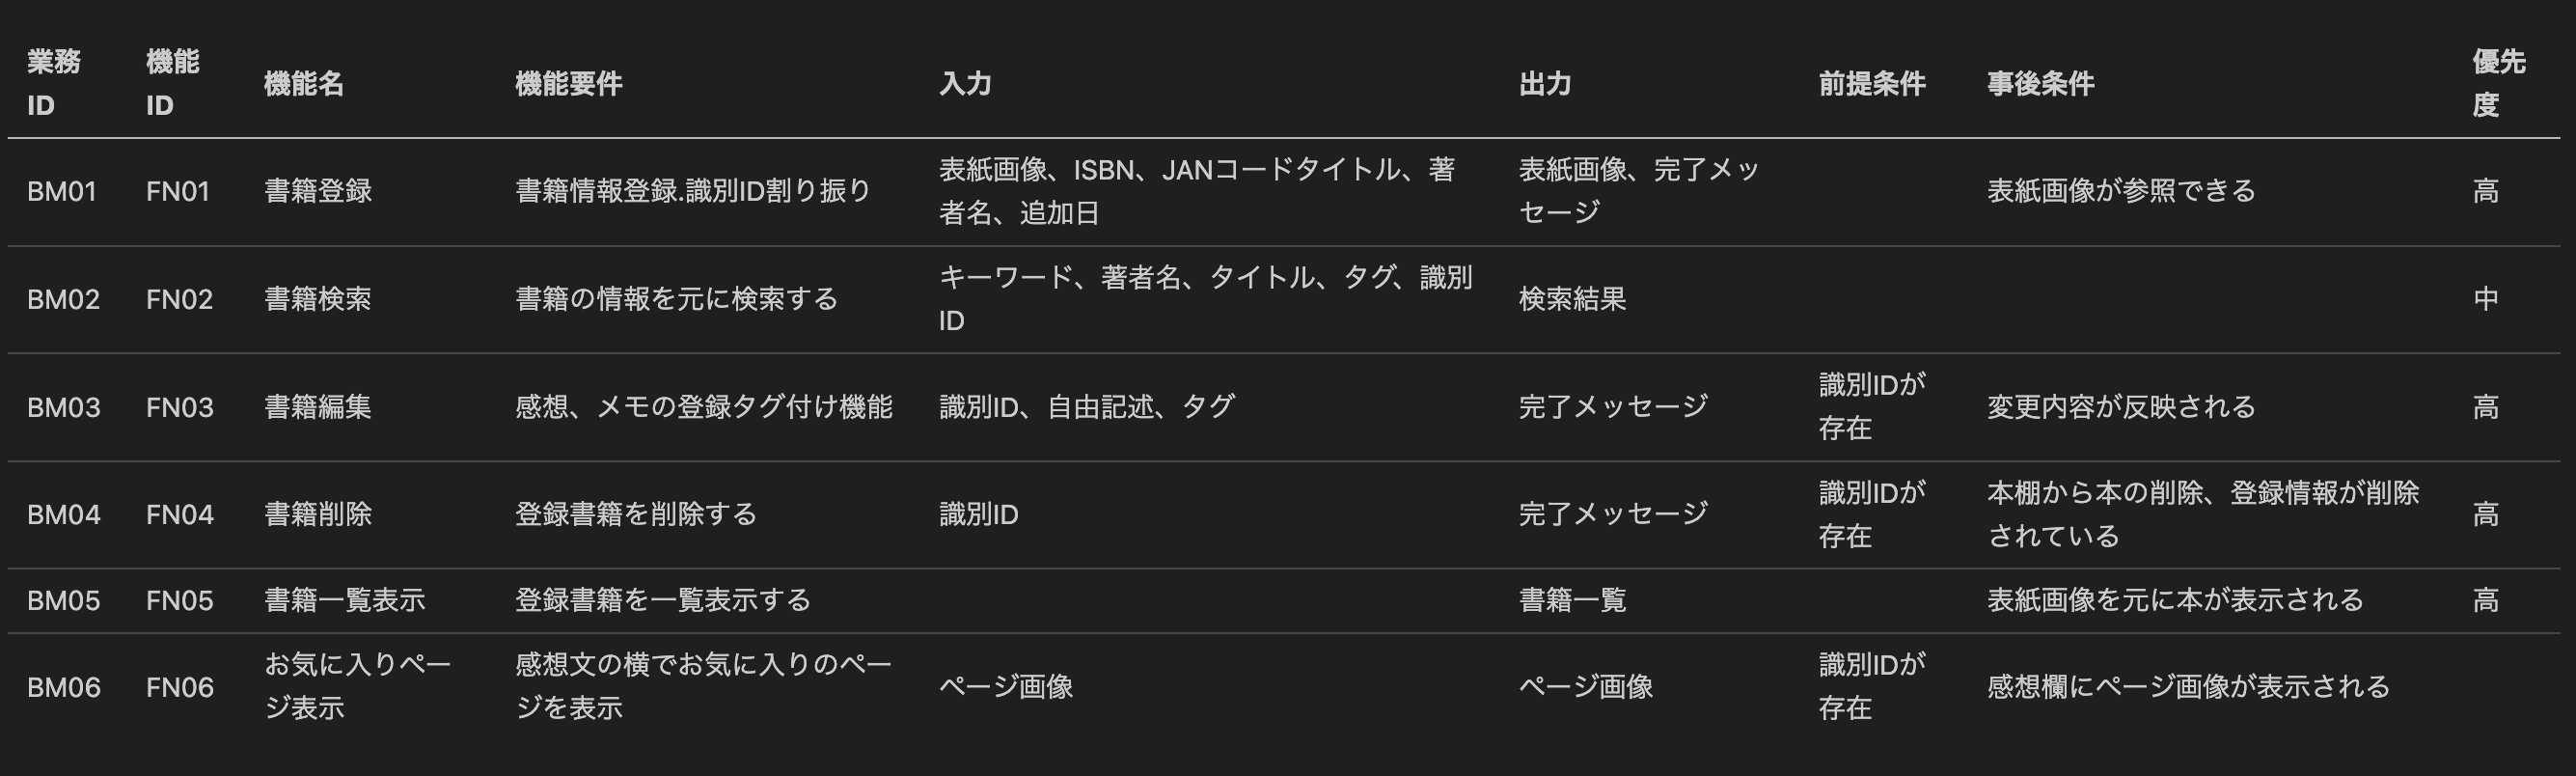
\includegraphics[width=120mm]{function.png}
\label{fig:func}
\end{figure}

\clearpage

\subsection{ワイヤーフレーム}
Figmaで作成。そのスクリーンショットを添付する。
\begin{figure}[htbp]
\centering
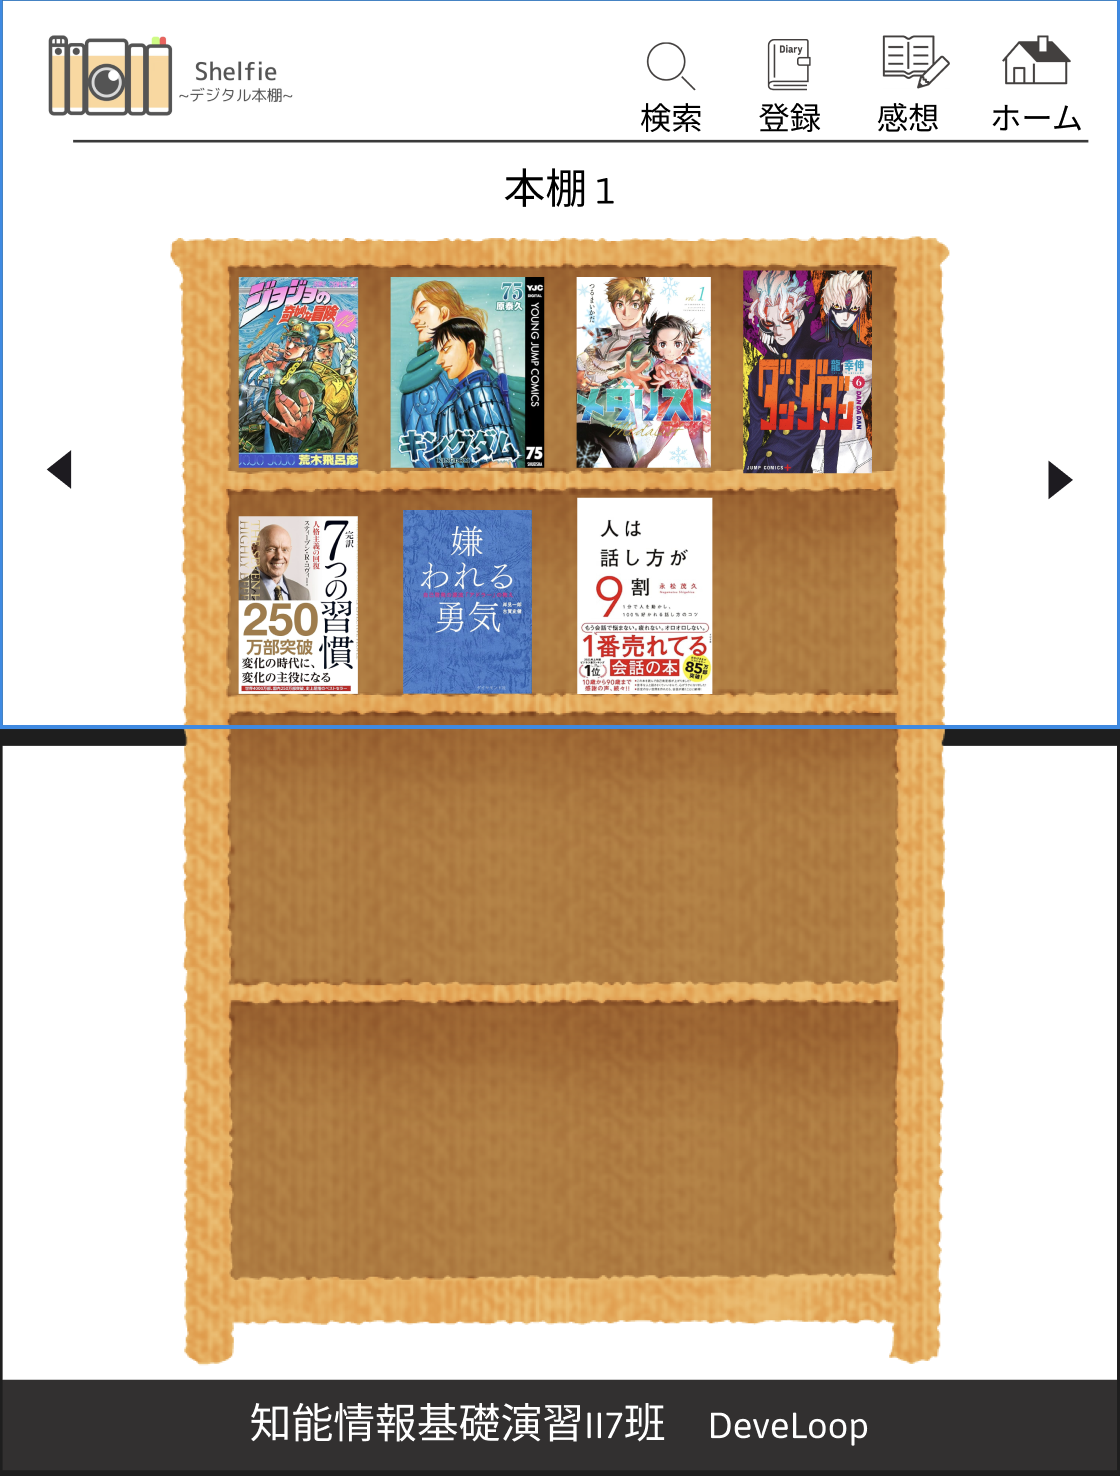
\includegraphics[width=120mm]{toppage.png}
\caption{トップページ}
\label{fig:func}
\end{figure}

\begin{figure}[htbp]
\centering
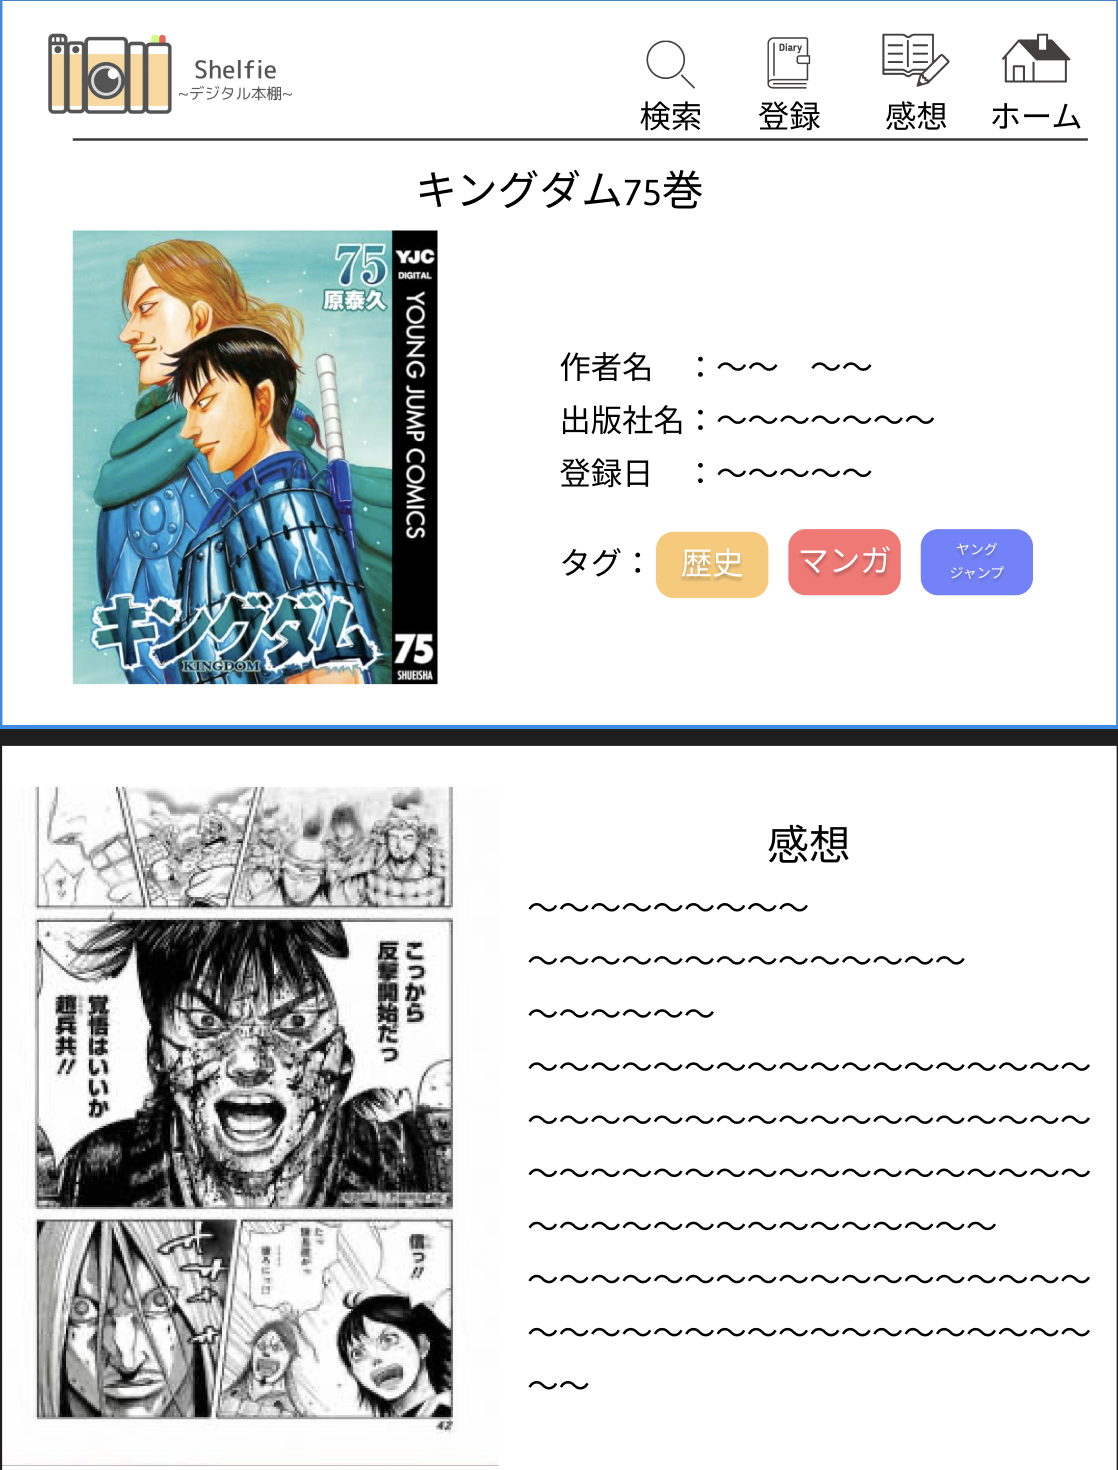
\includegraphics[width=120mm]{detailpage.png}
\caption{本の詳細ページ}
\label{fig:func}
\end{figure}

\subsection{ユースケース}
MIROで作成。そのスクリーンショットを添付する
\begin{figure}[htbp]
\centering
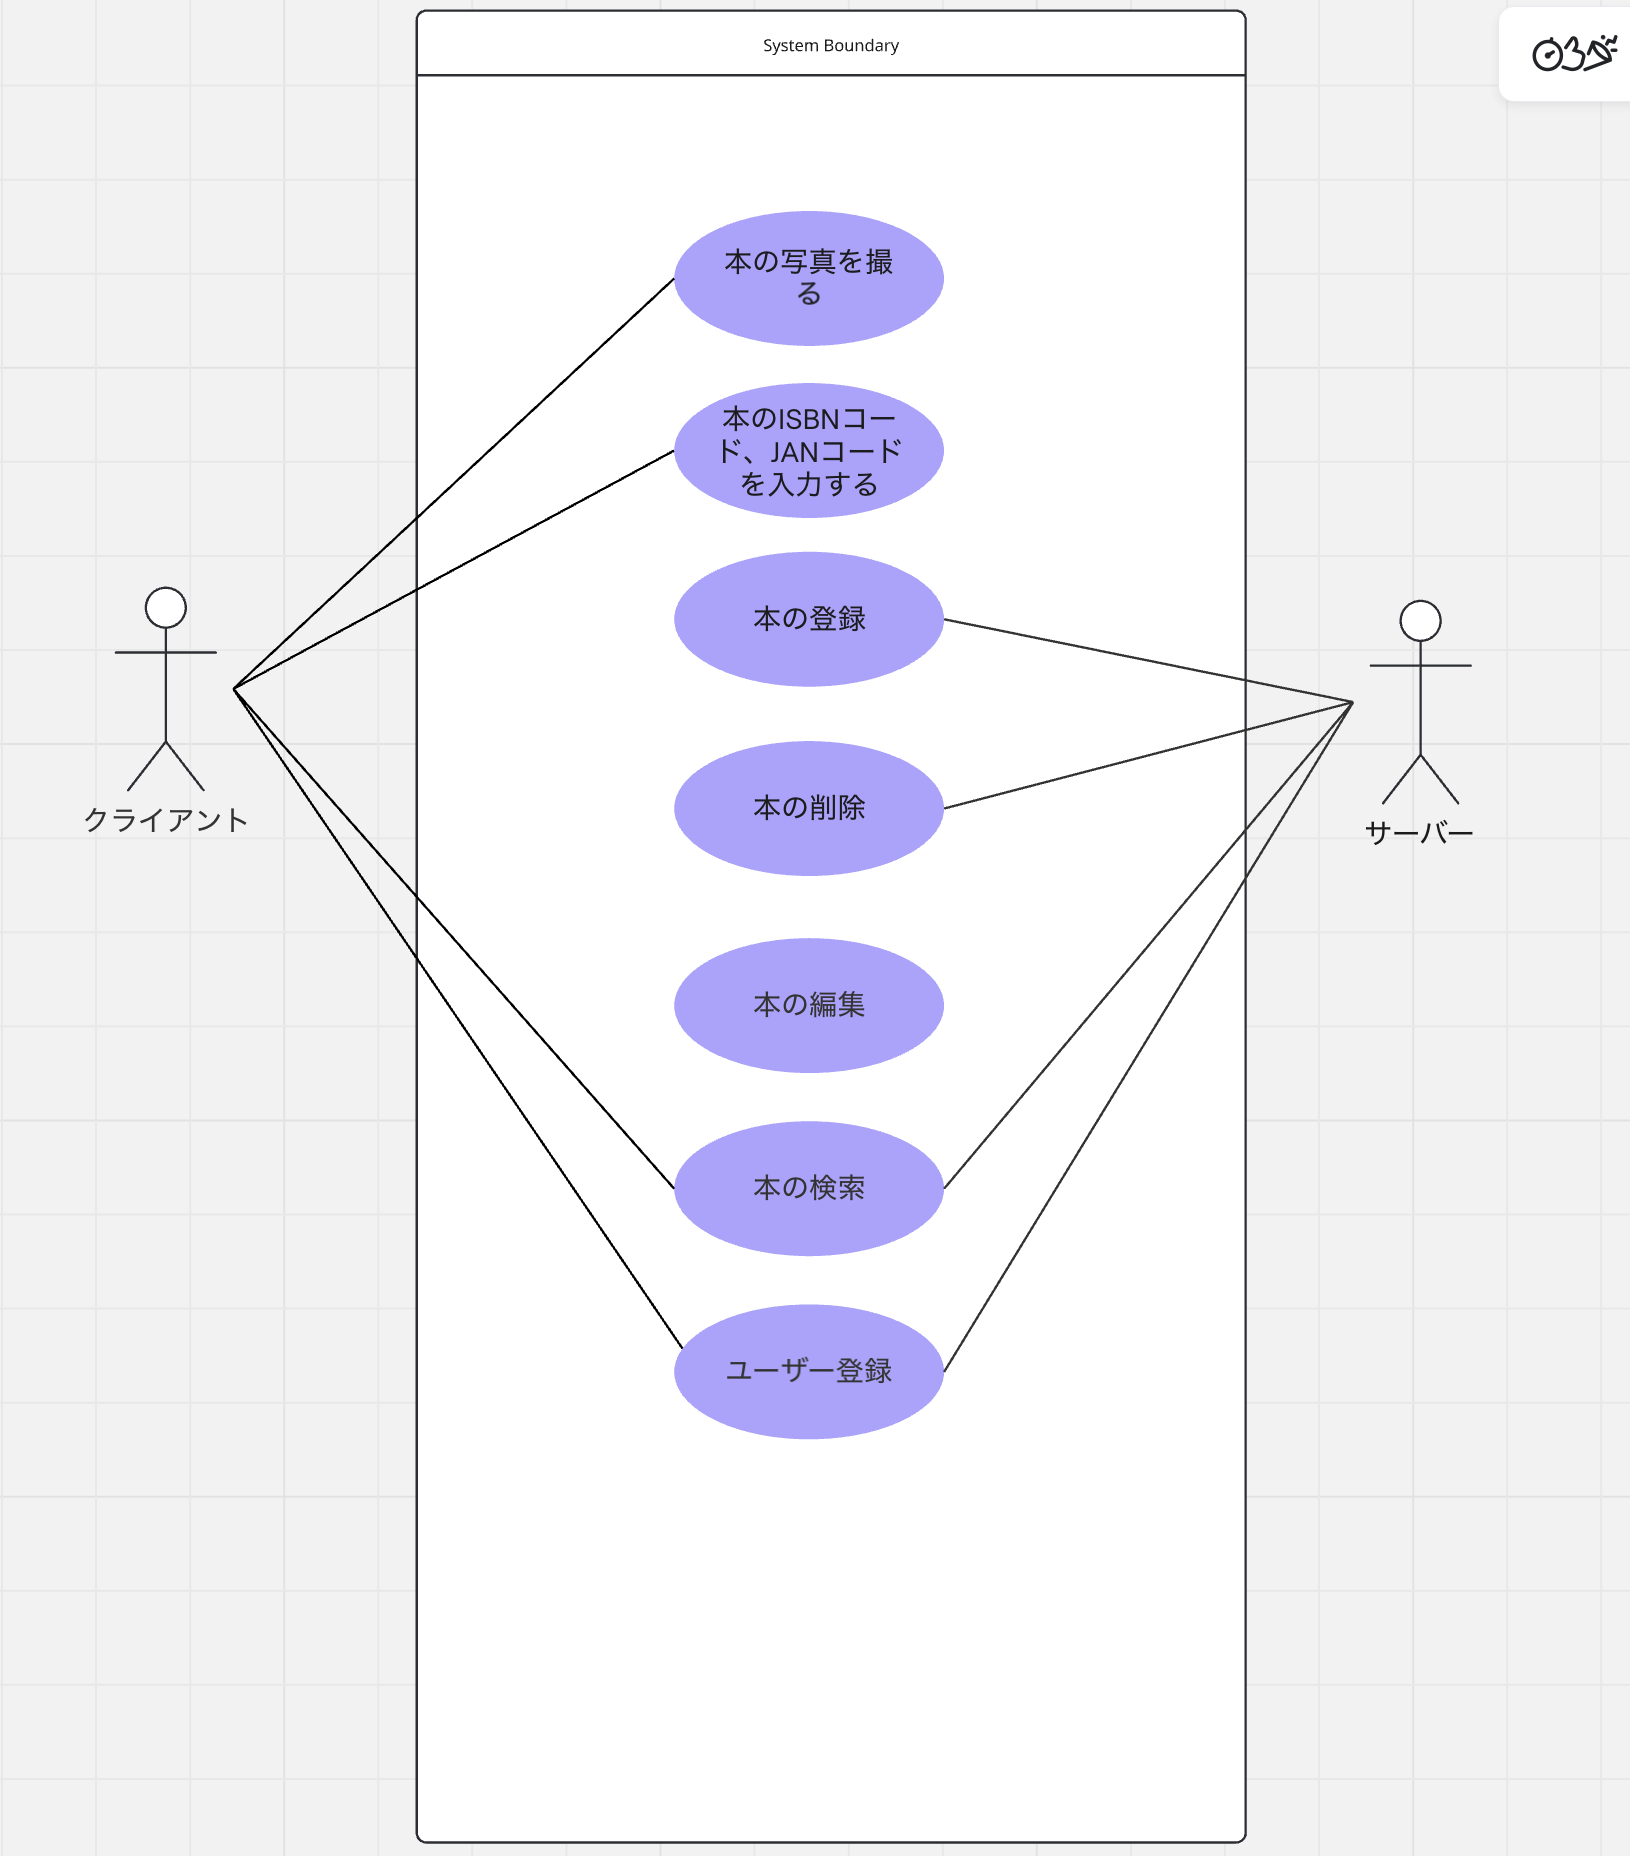
\includegraphics[width=120mm]{usecase.png}
\label{fig:func}
\end{figure}

\section{詳細設計書}

\subsection{開発環境・ツール}
\begin{itemize}
  \item 使用する言語
  \begin{itemize}
    \item フロントエンド\\
    HTML(Jinja2), CSS
    \item バックエンド\\
    Python3
  \end{itemize}
  \item フレームワーク\\
  Flask
  \item 開発ツール\\
  VSC
  \item バージョン管理システム\\
  Git, GitHub
\end{itemize}

\subsection{システム構成}
\begin{figure}[htbp]
\centering
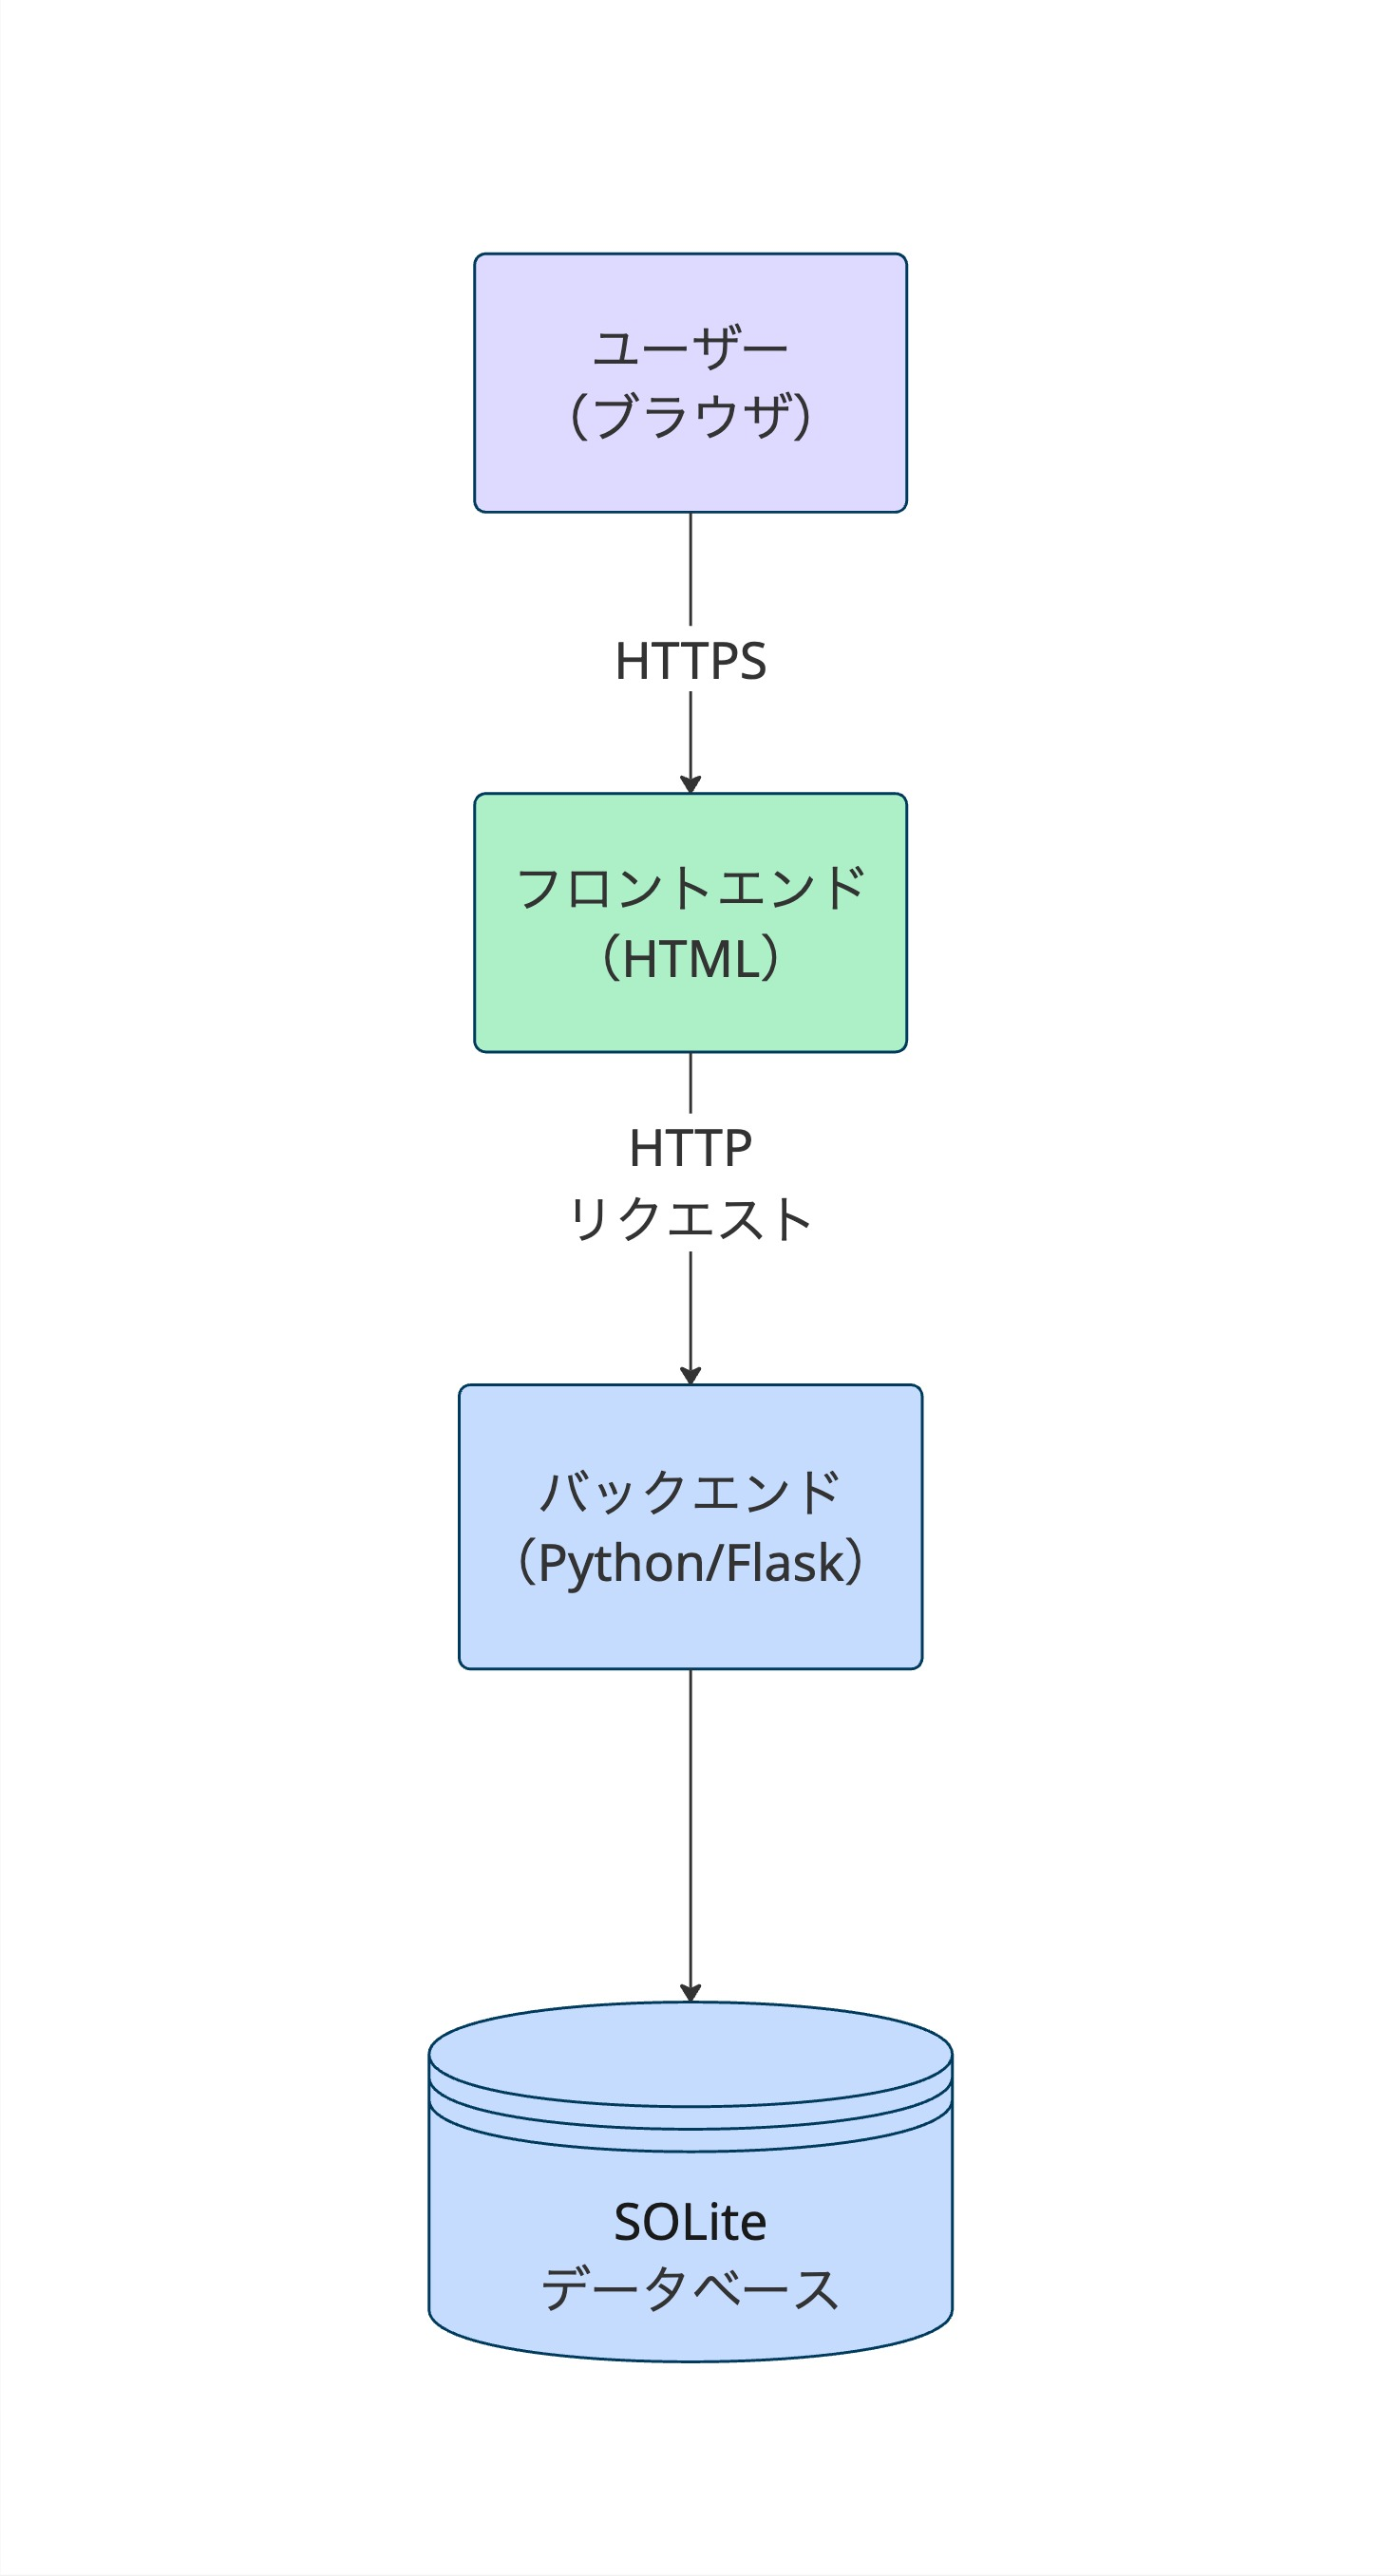
\includegraphics[width=70mm]{systemStructure.jpg}
\label{fig:func}
\end{figure}

\subsection{データベース設計}
\subsubsection{ブックテーブル(book)}
\begin{figure}[htbp]
\centering
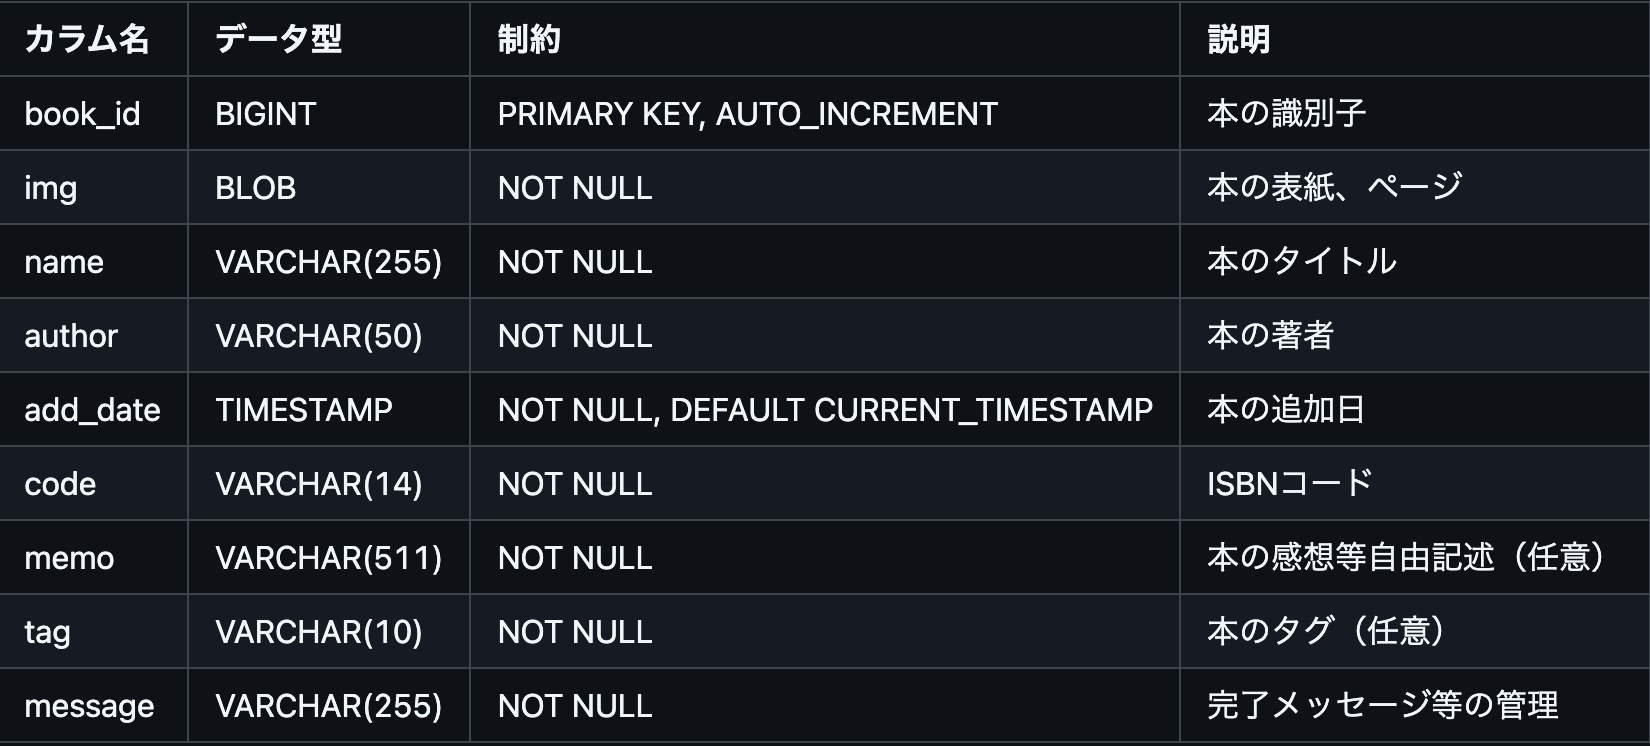
\includegraphics[width=120mm]{databasebook.png}
\label{fig:func}
\end{figure}

\subsubsection{本棚テーブル(shelf)}
\begin{figure}[htbp]
\centering
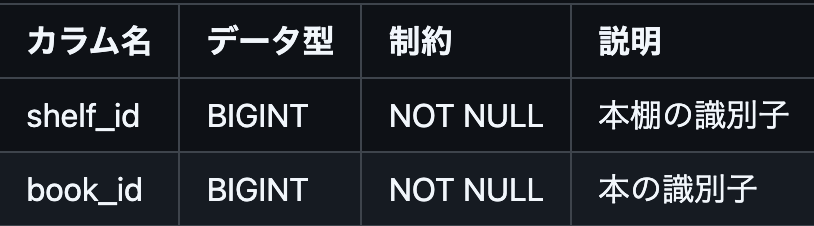
\includegraphics[width=120mm]{databaseshelf.png}
\label{fig:func}
\end{figure}

\clearpage
\subsection{各機能の処理フロー}
\subsubsection{書籍一覧表示}
\begin{figure}[h]
\centering
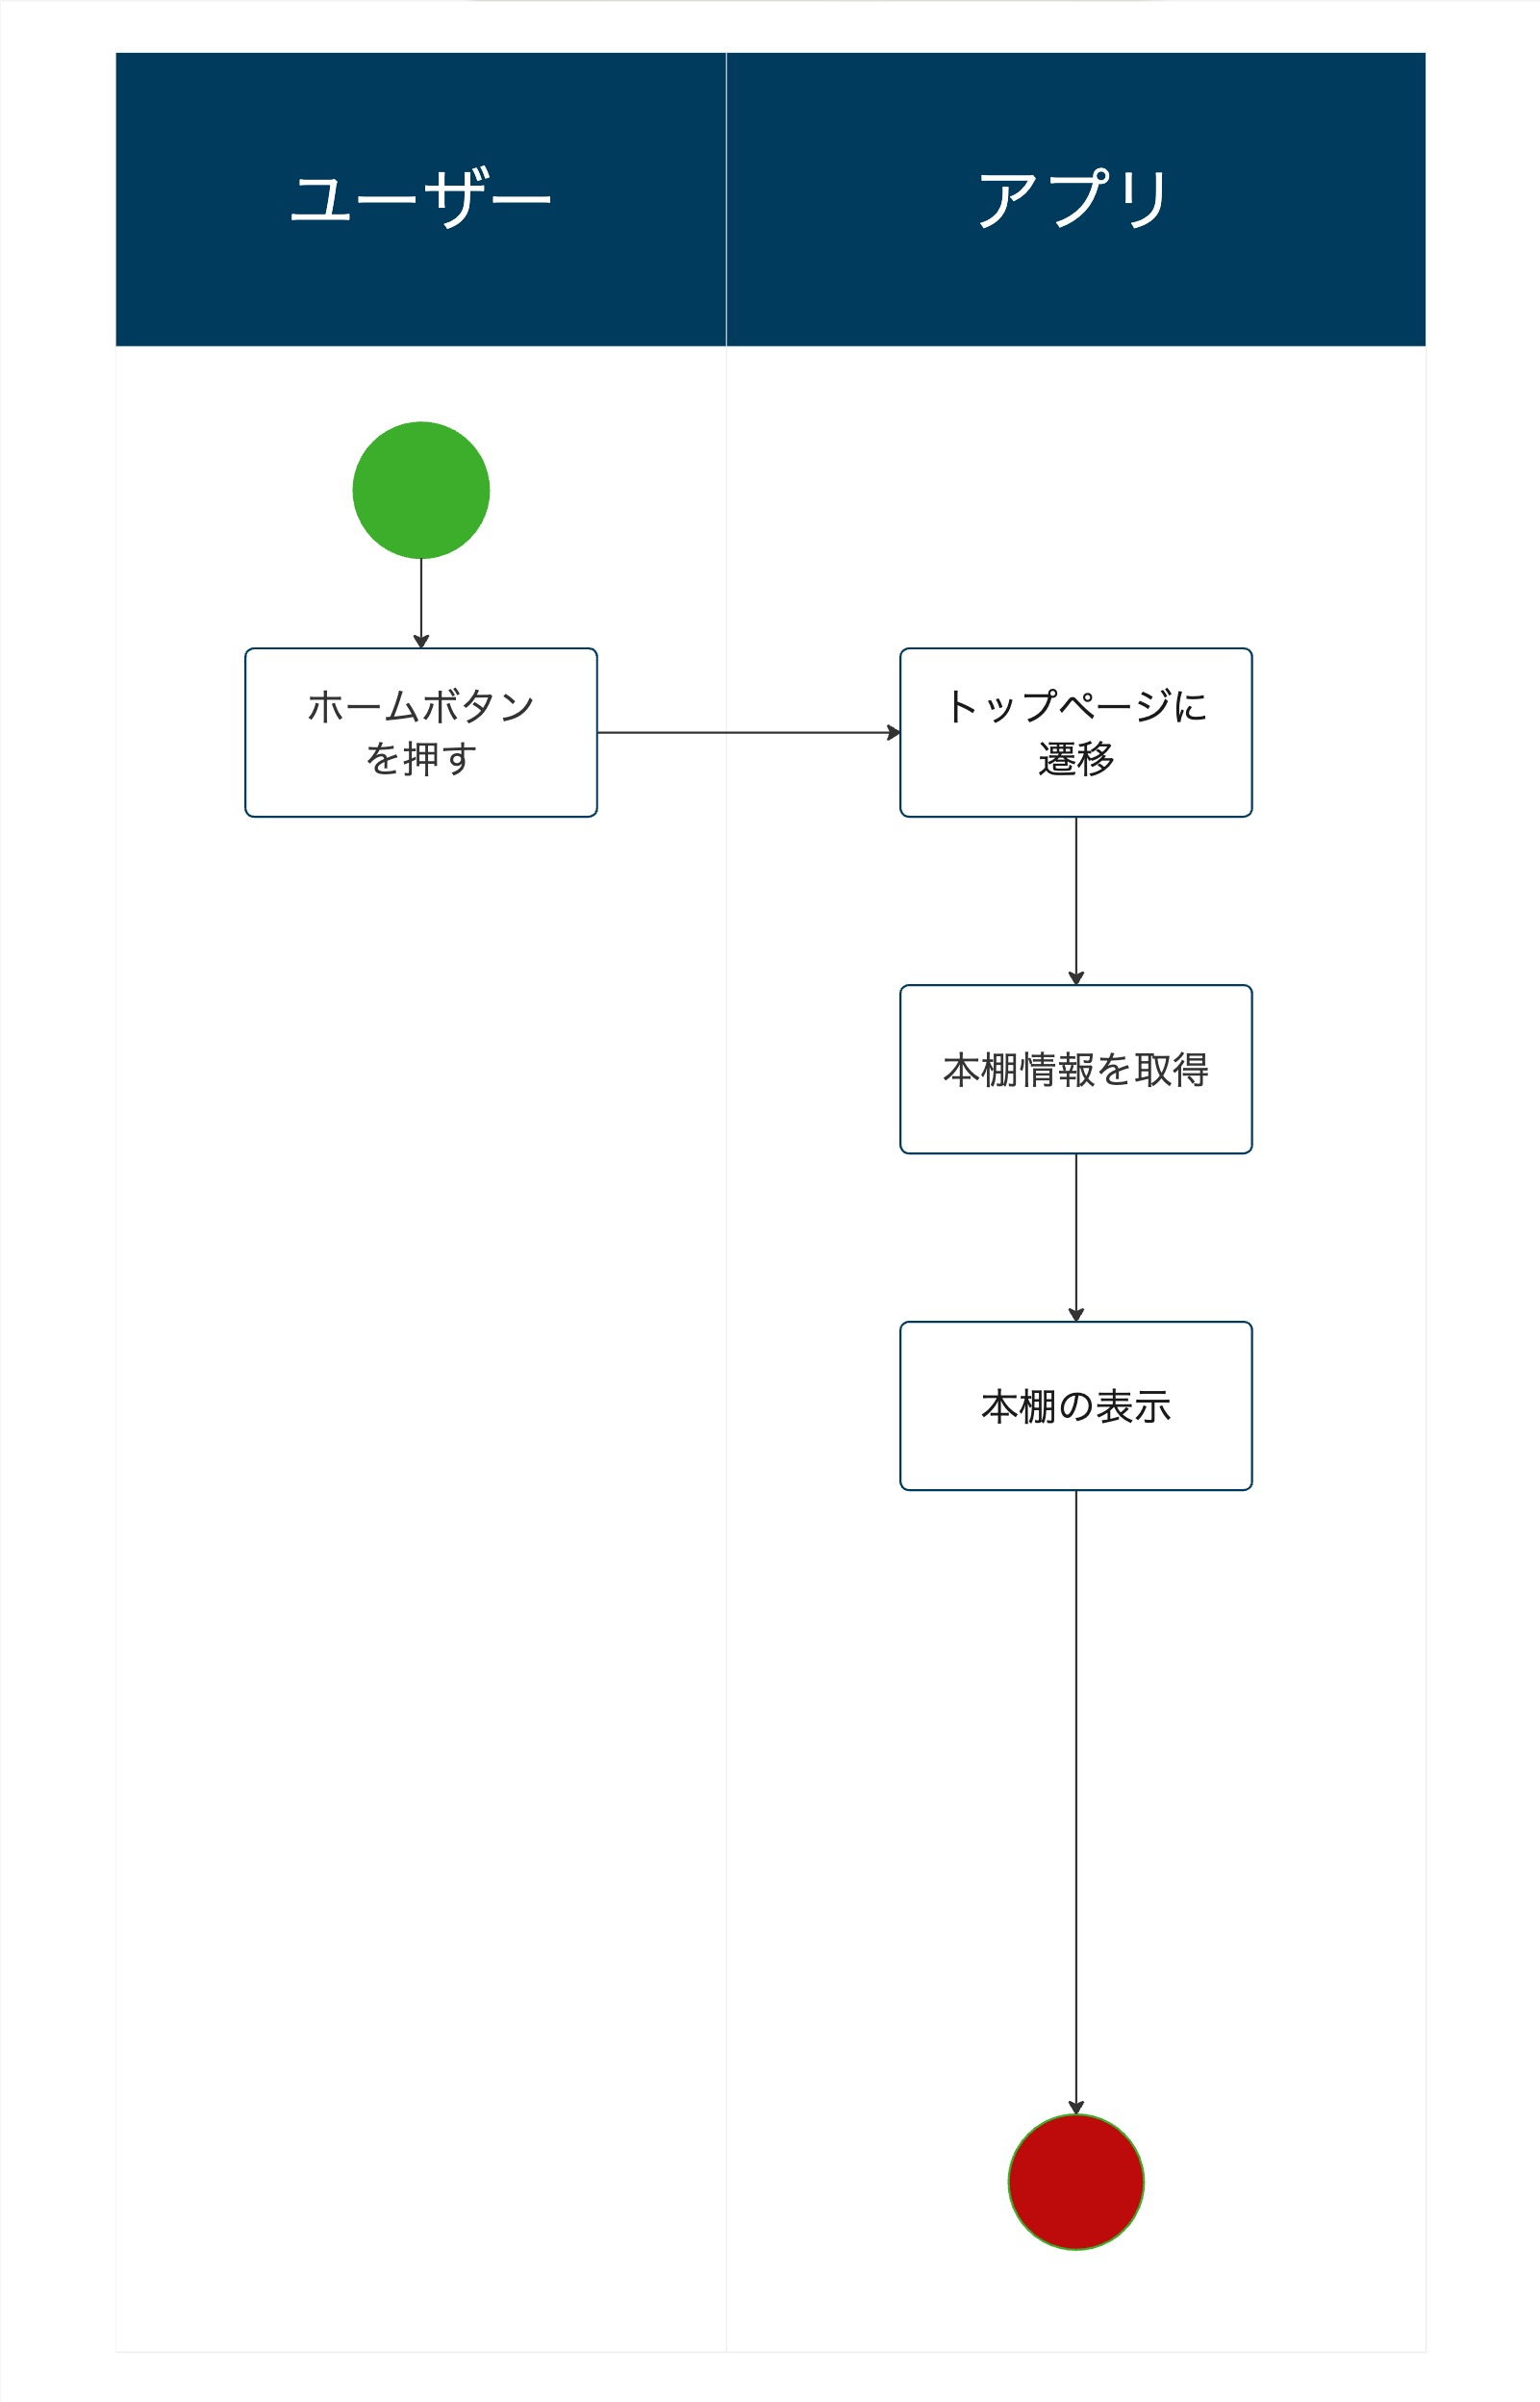
\includegraphics[width=100mm]{flow-ichiran.jpg}
\label{fig:func}
\end{figure}

\clearpage
\subsubsection{書籍登録}
\begin{figure}[h]
\centering
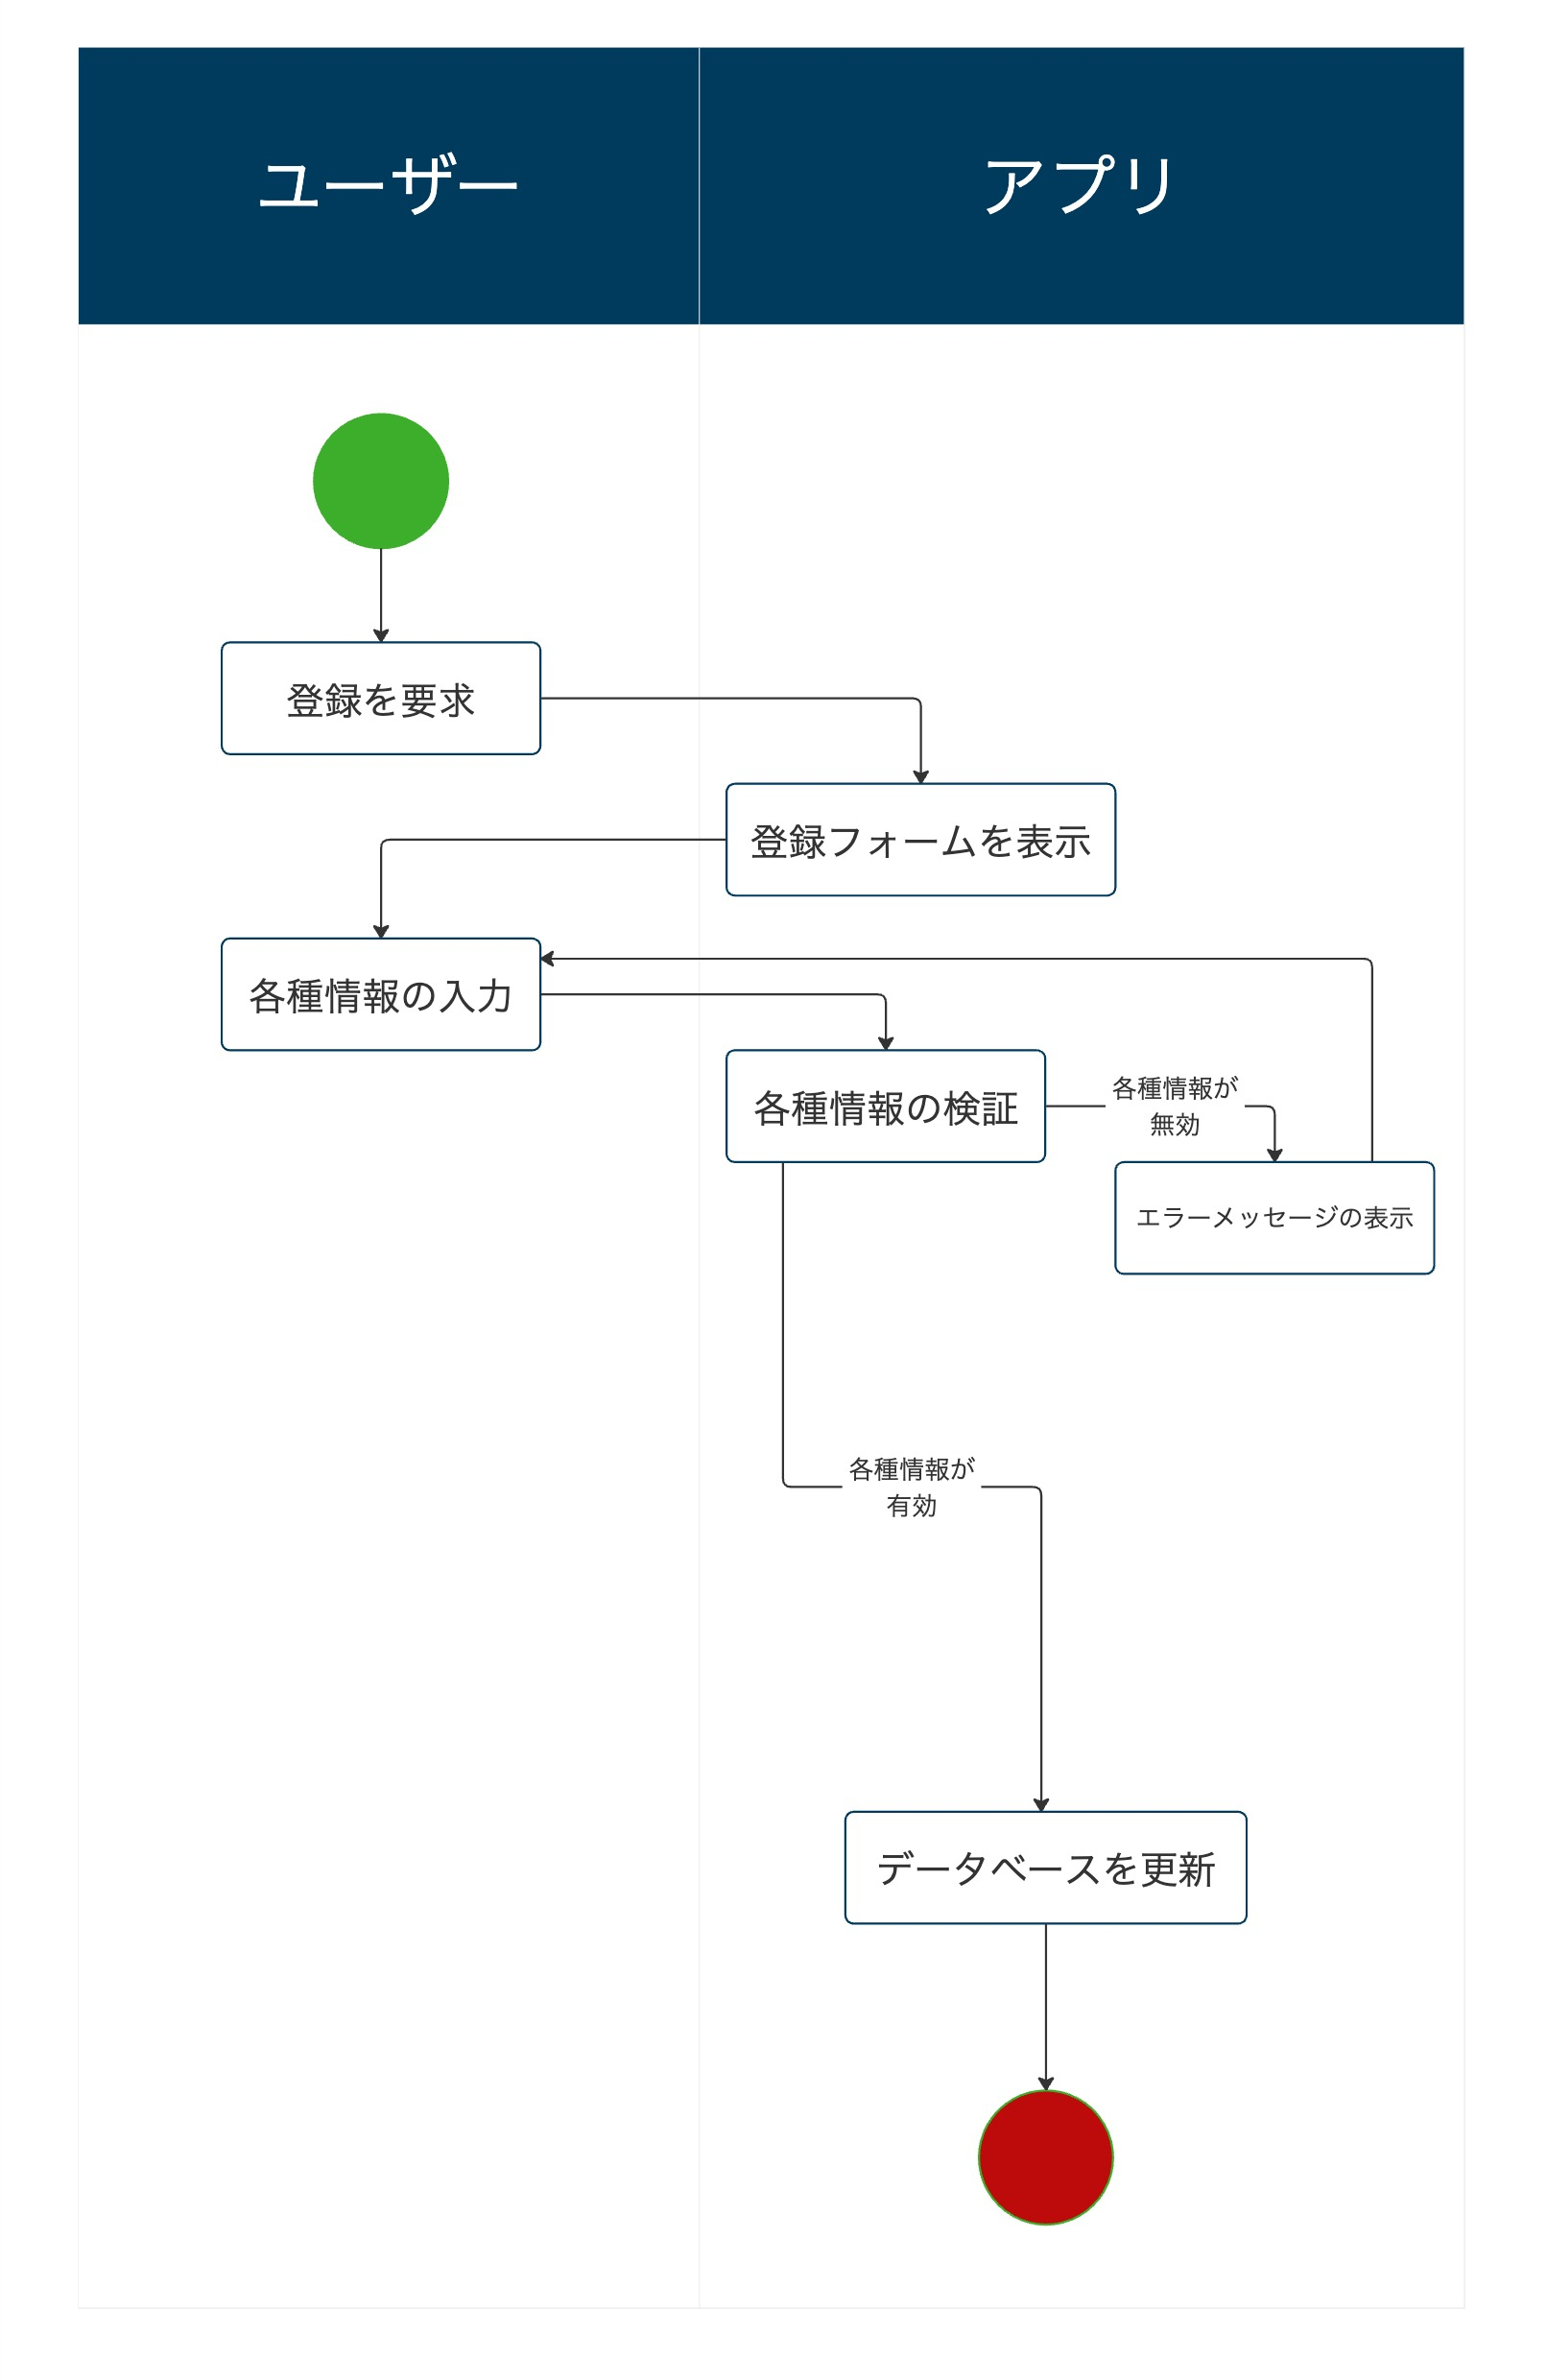
\includegraphics[width=100mm]{flow-touroku.jpg}
\label{fig:func}
\end{figure}

\clearpage
\subsubsection{書籍編集}
\begin{figure}[h]
\centering
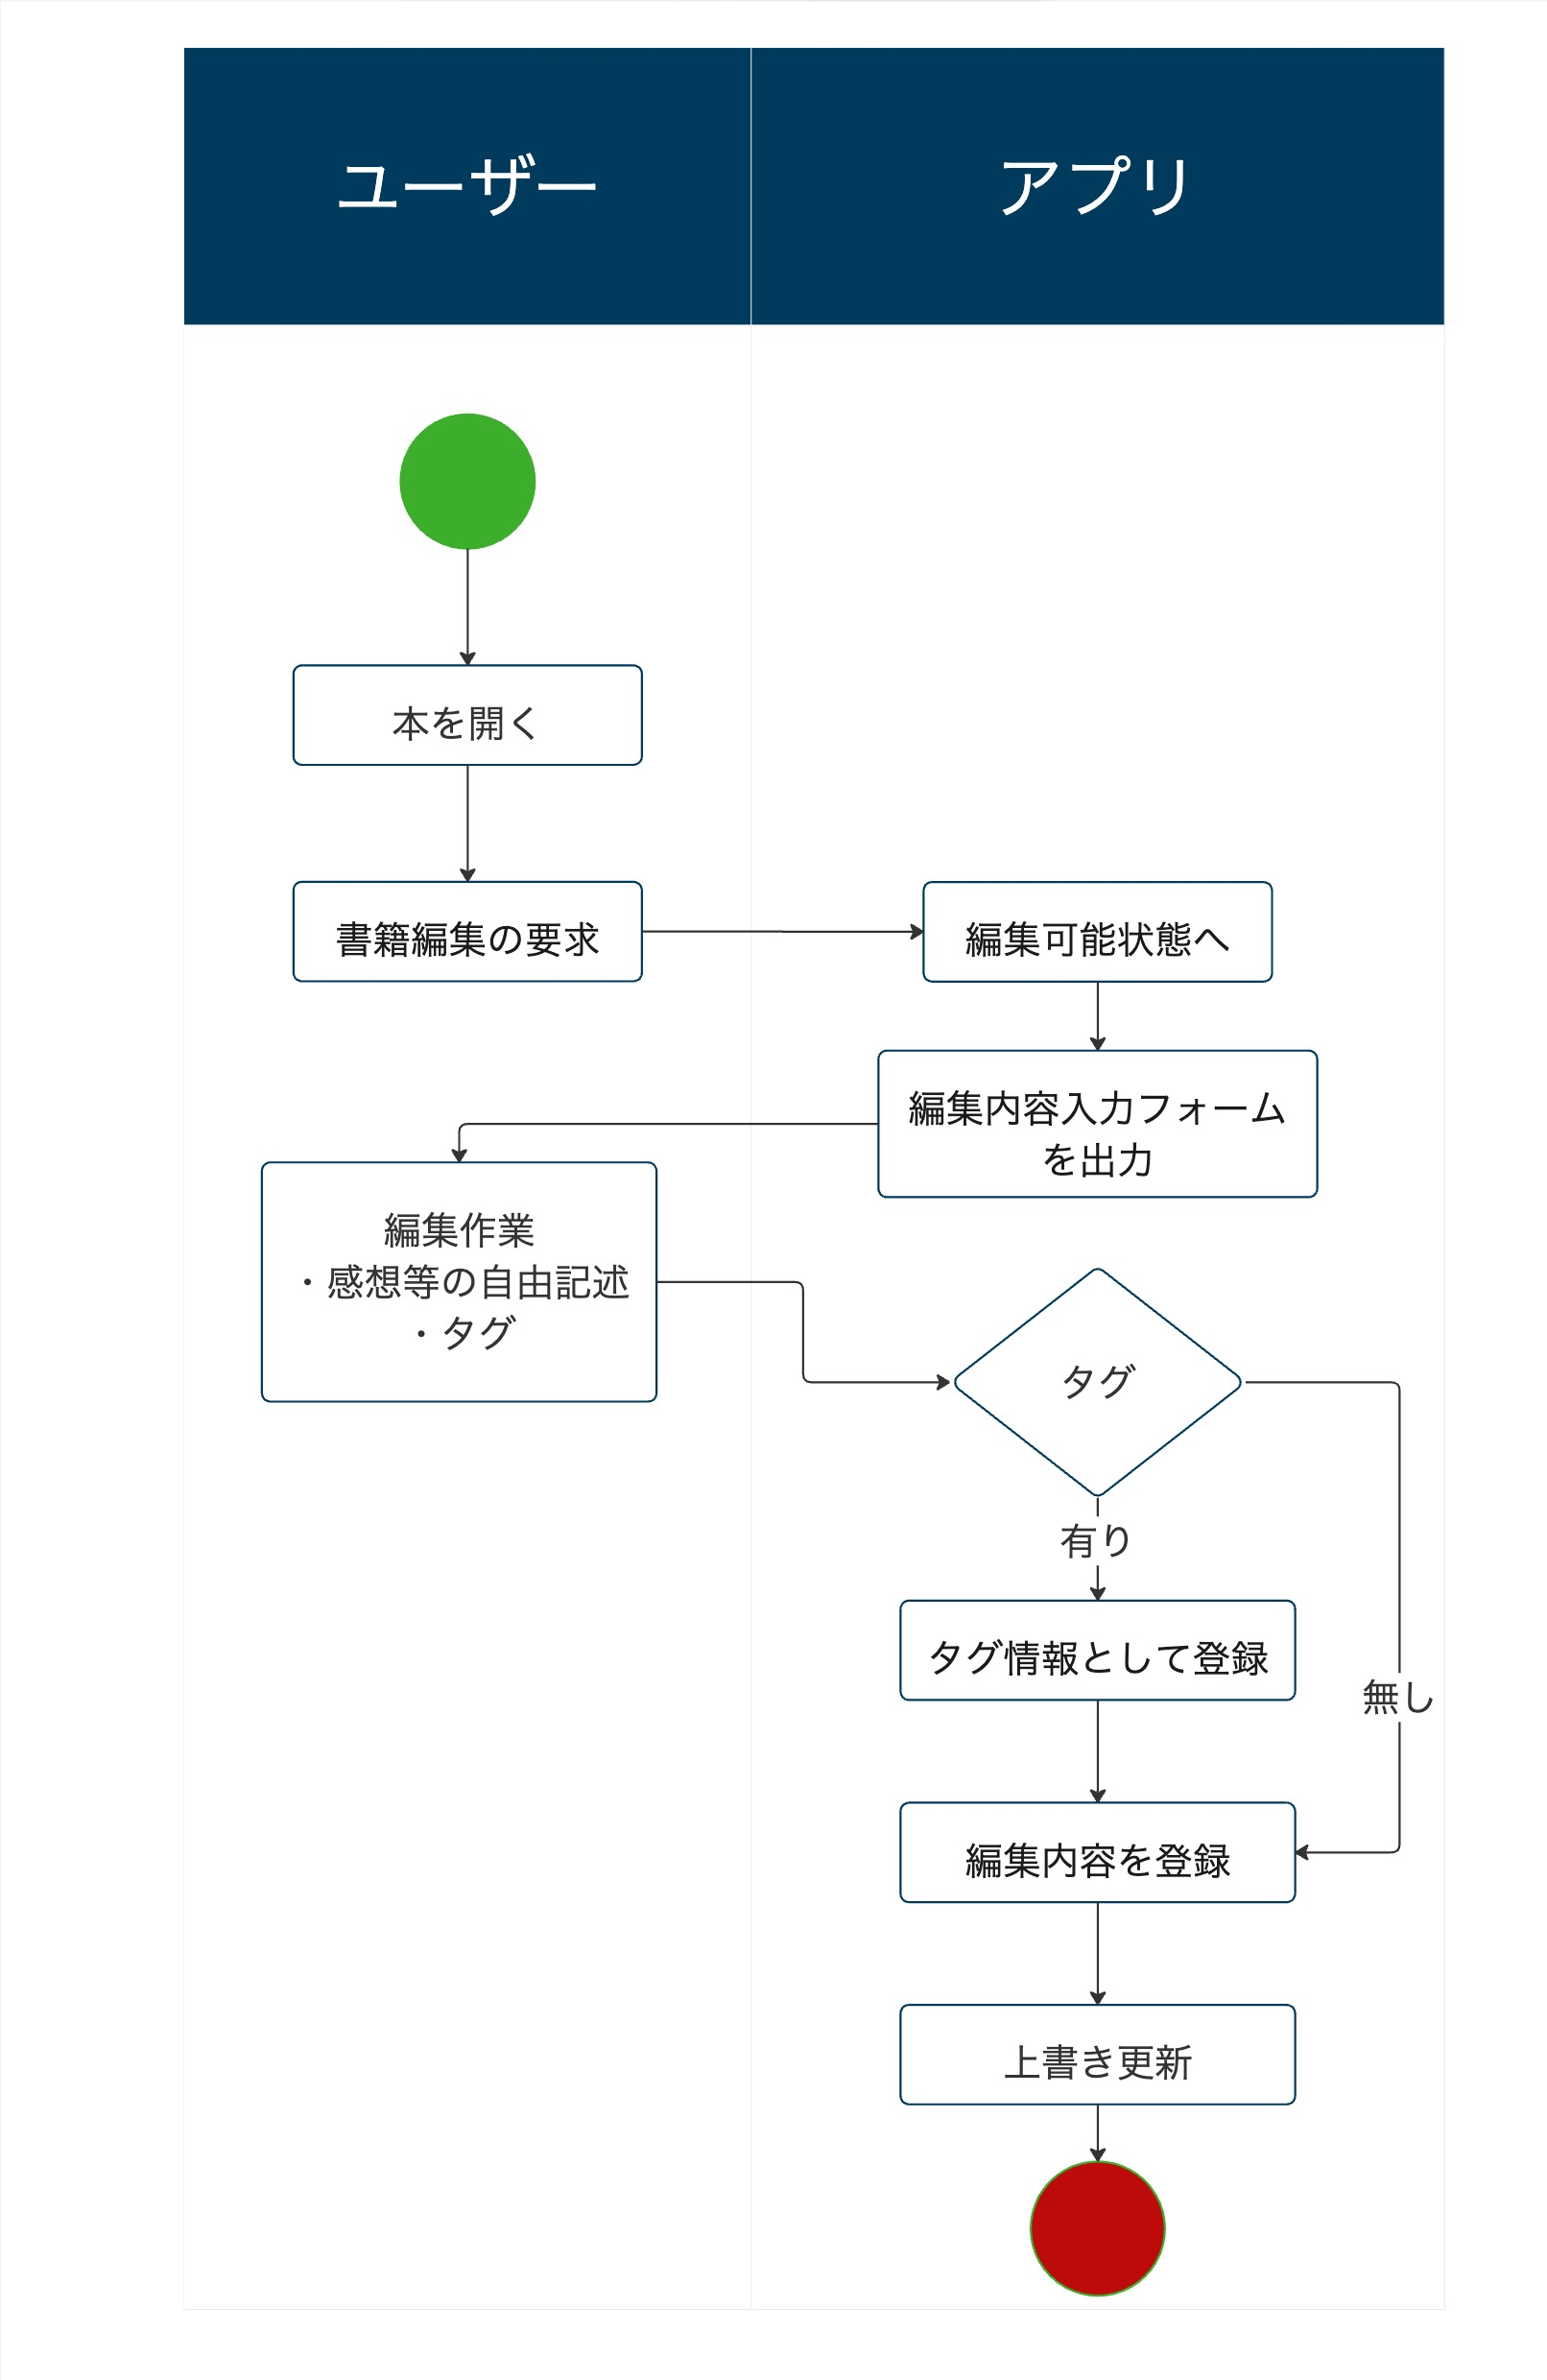
\includegraphics[width=100mm]{flow-henshu.jpg}
\label{fig:func}
\end{figure}

\section{グループでの分担内容と貢献度、MVP}%----------------------------------------------------------------------------------------------

\subsection{詳細設計書におけるグループでの分担内容と貢献度}
\begin{itemize}
    \item \textbf{245429H 末吉 良多(30\%)}開発環境・ツールと書籍一覧表示フローを作成。
    \item \textbf{245745J 知念 拓弥(40\%)}システム構成図と書籍登録フローを作成。とりまとめ。
    \item \textbf{245704B 武嶋 優海(30\%)}データベース設計と書籍編集フローを作成。
\end{itemize}

\textbf{MVP : 245745J 知念拓弥}

\end{document}